\section{Problema 3: La comunidad del anillo}

\subsection{Presentación del problema}

Dado un conjunto de computadoras, y un conjunto de enlaces entre pares de ellas (con a lo sumo un enlace para cada par), los cuales tienen un costo asociado, se pide elegir un conjunto de ellos tales que haya una red en forma ``anillo'', y que todas las computadoras tengan acceso a éste anillo usando enlaces de manera directa o indirecta (es decir, no es necesario que tengan un enlace a una computadora del anillo, sino que pueden tenerlo con una computadora intermedia), de manera de minimizar el costo total de los enlaces elegidos. Veamos por ejemplo las siguientes dos figuras:

\begin{figure}[ht]
	\begin{minipage}[t]{0.5\linewidth}
		\centering
		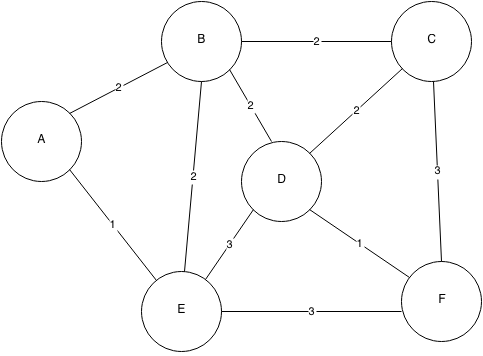
\includegraphics[width=\textwidth]{ej3_ejemplo.png}
		\caption{Red original}
		\label{fig:ej3_ejemplo}
	\end{minipage}
	\begin{minipage}[t]{0.5\linewidth}
		\centering
		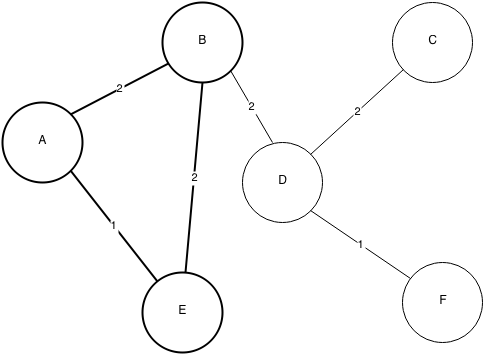
\includegraphics[width=\textwidth]{ej3_ejemplo_solucion_optima.png}
		\caption{Una solución óptima}
		\label{fig:ej3_ejemplo_solucion_optima}
	\end{minipage}
\end{figure}

En la Figura \ref{fig:ej3_ejemplo} vemos una red de seis computadoras con sus enlaces y sus costos asociados, y en la Figura \ref{fig:ej3_ejemplo_solucion_optima} tenemos una solución óptima del problema, con el anillo de equipos remarcado.

\subsection{Resolución}

Primero necesitamos caracterizar al conjunto de soluciones del problema. Como a lo sumo hay un enlace entre dos máquinas, podemos pensar a éstas como vértices, y a los enlaces como aristas. Entonces, tenemos como input un grafo $G = (V,X)$, y una solución (si existe) será un subgrafo de $G$ con las siguientes características:
\begin{enumerate}
    \item Debe ser \textbf{generador}, ya que para toda computadora se cumple que: o forma parte del anillo, o existe un camino simple que lleva a alguna máquina del anillo, y para ésto todas las computadoras deben estar en el subgrafo solución.
    \item Debe ser \textbf{conexo}, porque si no lo fuera, eso implica que hay alguna máquina que no puede conectarse con el anillo.
    \item Debe tener un \textbf{circuito simple}, éste será el anillo. Si no puede contruirse, no habrá solución.
    \item Más aún, debe tener \textbf{exactamente un circuito simple}. El problema no prohíbe que haya más de uno, pero si tuviéramos más de un ciclo, bastaría con quitar la arista más costosa que forme parte de algún circuito para mejorar la solución, ya que el subgrafo seguiría siendo conexo (los caminos simples que pasaran por la arista que quitamos podrían desviarse por el resto del circuito) y seguiría existiendo al menos un circuito simple (si no, este subgrafo sería un árbol, pero entonces agregar la arista que quitamos nos daría un grafo con exactamente un circuito simple, absurdo). Este procedimiento lo podríamos repetir hasta que sólo quede un circuito. Luego, podemos descartar todos los subgrafos con más de un circuito simple, ya que son soluciones necesariamente subóptimas.
\end{enumerate}
Tenemos entonces caracterizada a una solución como un subgrafo generador de $G$ conexo y con exactamente un circuito simple. Una solución óptima entonces será minimizar el costo de este tipo de subgrafos. Vamos a construir una solución óptima en dos pasos:
\begin{enumerate}
 \item Hallaremos $T = (V, X_T)$ un árbol generador mínimo de $G$ (si no existe, no hay solución).
 \item Tomaremos la arista $e$ de mínimo costo en $X - X_T$ (si el conjunto es vacío, no hay solución) y la agregaremos a $T$.
\end{enumerate}
Nuestro algoritmo construirá entonces el subgrafo $S = (V, X_T \cup \left\{e\right\})$. En la demostración de correctitud veremos que efectivamente $S$ es una solución óptima del problema.

Para obtener el árbol generador mínimo usamos el algoritmo de Prim, luego a este grafo le agregaremos la arista más chica de las que no pertenecen a él, y finalmente para encontrar el ciclo usaremos la función DFS\_visit, que hace un Depth-First Search sobre la solución para encontrar al único circuito simple.

La función DFS\_visit es la misma que la presentada en el libro de Cormen \emph{Introduction to Algorithms}\cite[p.~604]{cormen} añadiéndole la funcionalidad de distinguir un \emph{back edge} (esto es, una arista que efectivamente cierra un ciclo en el grafo). En el libro, se llama primero a la función DFS, que inicializa todos los vértices con color blanco (esto significa que no fueron visitados), y luego llama a DFS\_visit para cada uno de los vértices del grafo que tengan ese color. Como nuestro grafo solución es conexo, alcanza llamar a DFS\_visit con un sólo vértice para que DFS recorra todo el grafo. En particular, la llamaremos con un vértice que sabemos que está en el ciclo, esto es, con uno de los vértices en los que incide la arista que agregamos al final. Así, al finalizar DFS\_visit, como el vértice tendrá necesariamente un \emph{back edge}, lo usaremos para reconstruir el único ciclo (el \emph{back edge} es una arista del ciclo, y luego alcanza con pedir el anterior del otro vértice hasta que lleguemos al mismo con el que llamamos a DFS\_visit originalmente). 

La información que nos da DFS\_visit la guardamos en un array de la estructura infoVerticeDFS, donde la posición i-ésima corresponde al vértice i-ésimo. Este array inicializa todos los vértices en el color blanco. Luego, cada vez que visitamos un vértice, es decir, cada vez que se ejecuta DFS\_visit, el vértice se pone de color gris, hasta que se terminen de considerar sus vértices adyacentes. Una vez hecho esto, se pone de color negro. Entonces, si al visitar un vértice ocurre que entre sus adyacentes hay uno coloreado gris, y no es el anterior al actual (de lo contrario sería como volver por el mismo camino, lo cual no es un circuito simple), esto implica que la arista que conecta con ese vértice es un \emph{back edge} (porque como está gris, todavía estábamos recorriendo caminos que salían de ese vértice, y volvimos a él), lo cual guardaremos en la información del vértice ya visitado. Por lo tanto, si la primera vez que llamamos a DFS\_visit lo hacemos con un vértice del circuito, necesariamente tendremos su único \emph{back edge} al finalizar.

\subsubsection{Pseudocódigo}

\begin{algorithm}[H]
\begin{algorithmic}[1]
\caption{LaComunidadDelAnillo(aristasGrafo)}
\STATE Conjunto(Vertice) verticesAGM $\leftarrow$ vacía
\STATE Conjunto(Arista) aristasAGM $\leftarrow$ vacía
\STATE Conjunto(Arista) aristasCandidatasAGM $\leftarrow$ vacía
\STATE Pongo el vértice 0 en verticesAGM, y sus aristas en aristasCandidatasAGM
\WHILE {$|$aristasAGM$|$ $<$ n - 1 \AND $|$aristasCandidatasAGM$|$ $>$ 0}
	\STATE Tomar la arista candidata de menor costo (quitándola además de las candidatas)
    \IF {La arista incide en dos vértices del AGM}
        \STATE No la puedo usar
    \ELSE
        \STATE Insertar el nuevo vértice en verticesAGM
        \STATE Eliminar la arista de aristasGrafo
        \STATE Insertar la arista en aristasAGM
        \FOR {\textbf{each} arista del nuevo vértice (que no fue considerada antes)}
            \STATE Insertar arista en aristasCandidatasAGM
        \ENDFOR
    \ENDIF
\ENDWHILE
\IF {$|$aristasAGM$|$ $<$ n - 1 \OR $|$aristasGrafo$|$ == 0}
    \STATE No hay solución
\ENDIF
\STATE Arista aristaMenor $\leftarrow$ Arista de menor costo de aristasGrafo
\STATE Vertice primero $\leftarrow$ El primer vértice de aristaMenor (podría ser cualquiera de los dos vértices, no afecta al algoritmo)
\STATE Insertar aristaMenor en aristasAGM
\STATE infoVerticeDFS info$[$n$]$ \textcolor{CadetBlue}{// Ésto tiene la información del recorrido DFS, se inicializan los vértices en BLANCO}
\STATE Llamar a la función DFS\_visit(info, primero) sobre el subgrafo solución
\STATE Arista backEdge $\leftarrow$ info[primero].backEdges.front()
\STATE Lista(Arista) aristasAnillo $\leftarrow$ vacía
\STATE Insertar backEdge en aristasAnillo
\STATE Eliminar backEdge de aristasAGM
\STATE Vertice actual $\leftarrow$ backEdge.dameElOtroVertice(primero)
\WHILE {actual $\neq$ primero}
    \STATE Eliminar info[actual].aristaAnterior de aristasAGM
    \STATE Insertar info[actual].aristaAnterior en aristasAnillo
    \STATE actual $\leftarrow$ info[actual].verticeAnterior
\ENDWHILE
\end{algorithmic}
\end{algorithm}

Al finalizar el algoritmo, las aristas del circuito de la solución óptima quedan en $aristasAnillo$, y el resto en $aristasAGM$.

\begin{algorithm}[H]
\begin{algorithmic}[1]
\caption{DFS\_visit(infoVerticeDFS * info, Vertice actual)}
\STATE info[actual].estado $\leftarrow$ GRIS
\FOR {\textbf{each} arista del vértice actual}
    \STATE Vertice nuevoActual $\leftarrow$ arista.dameElOtroVertice(actual)
    \IF {info[nuevoActual].estado == BLANCO}
        \STATE info[nuevoActual].aristaAnterior $\leftarrow$ arista
        \STATE info[nuevoActual].verticeAnterior $\leftarrow$ actual
        \STATE DFS\_visit(aristasDeCadaVerticeAGM, info, nuevoActual)
    \ELSIF {info[nuevoActual].estado == GRIS}
        \IF {nuevoActual == info[actual].verticeAnterior}
            \STATE \textcolor{CadetBlue}{// Si estoy acá es porque estaba volviendo por la misma arista que vine (formando un circuito NO simple)}
        \ELSE
            \STATE \textcolor{CadetBlue}{// El nuevo vertice ya habia sido visitado, entonces hay back edge}
            \STATE Insertar arista en info[nuevoActual].backEdges
        \ENDIF
    \ENDIF
\ENDFOR
\STATE info[actual].estado $\leftarrow$ NEGRO
\end{algorithmic}
\end{algorithm}

\subsection{Demostración}

Nuestro algoritmo encuentra un árbol generador mínimo del grafo de la red de computadoras, y le añade la arista (conexión) más barata de las que quedaron. Afirmamos que ésa es una solución óptima para el problema. Podemos caracterizar toda solución como un grafo conexo con exactamente un circuito simple, siendo el circuito el ``anillo'' y el resto de las aristas las conexiones restantes. Como el grafo es conexo, todas las computadoras estarán conectadas, por lo tanto se cumple con lo pedido.

Veamos entonces que nuestro algoritmo devuelve una solución óptima. Demostraremos ésto por el absurdo, suponiendo que hay una solución estrictamente mejor que la nuestra. Pero primero, necesitamos demostrar el siguiente lema.

\begin{lema}
\label{lema_ej3}
Sea $G = (V,X)$ un grafo conexo con exactamente un circuito simple $C$. Sea $e$ una arista tal que $e \in C$. Sea $X' = X - \left\{e\right\}$. Entonces $G' = (V,X')$ es un árbol generador de $G$.
\end{lema}
\begin{proof}
Supongamos que $G' = (V,X')$ no es un árbol generador de $G$. Esto es, $G'$ no es generador de $G$, o no es árbol. \\
Si no fuera generador, entonces no tendría los mismos nodos que $G$, lo cual es absurdo porque $G = (V,X)$ y $G' = (V,X')$.
Entonces $G'$ no debe ser árbol. Esto es, o $G'$ no es conexo, o tiene al menos un circuito simple. \\
Si $G'$ no fuera conexo, entonces existen vértices $v$, $w$ en $V$ tales que no existe un camino simple entre ellos. Sabemos que $G$ es conexo, entonces sea $C_{v,w}$ el camino simple entre $v$ y $w$ partiendo desde $v$. Hay dos posibilidades: $e \in C_{v,w}$ ó $e \notin C_{v,w}$. 
\begin{itemize}
\item Si $e \notin C_{v,w}$, entonces $C_{v,w} \subseteq X'$ y por lo tanto el camino está en $G'$. 
\item Si $e \in C_{v,w}$, entonces $C_{v,w} \not\subseteq X'$, pero como $e \in C$, es decir, $e$ está en el circuito simple de $G$, si $e = (a,b)$ donde $a, b \in V$, entonces existen dos caminos entre $a$ y $b$, a saber: ir por $e$ ó ir por $C - \left\{e\right\}$. Podemos escribir $C_{v,w} = C_{v,a} \oplus (a,b) \oplus C_{b,w}$ donde $C_{v,a}$ y $C_{b,w}$ son los subcaminos entre $v$,$a$ y $b$,$w$ respectivamente, y además $e \notin C_{v,a}$, $e \notin C_{b,w}$ porque $C_{v,w}$ es camino simple. El camino $C'_{v,w} = C_{v,a} \oplus (C - \left\{e\right\}) \oplus C_{b,w}$ es un camino entre $v$ y $w$ tal que $C'_{v,w} \subseteq X'$, y por lo tanto hay un camino simple entre $v$ y $w$ en $G'$ (si $C'_{v,w}$ no fuera simple, siempre podemos quitar los circuitos que se generan al pasar por un mismo nodo, quedando de esa forma un camino simple).
\end{itemize}
Luego, $G'$ es conexo. Entonces $G'$ debe tener al menos un circuito simple $C'$, y $e \notin C'$ porque $e \notin X'$. Pero esto implica que $G$ tiene dos circuitos simples distintos porque $C' \subseteq X' \subseteq X$, y $C' \neq C$ pues $e \in C$, lo cual es absurdo porque por hipótesis $G$ tiene exactamente un circuito simple. El absurdo provino de suponer que $G'$ no es árbol generador de $G$. \\ Por lo tanto, $G'$ es un árbol generador de $G$.
\end{proof}

\begin{notacion}
Dado un grafo cualquiera $G = (V,X)$ con $x \in X$, 
\begin{align*}
G - \left\{x\right\} = (V, X - \left\{x\right\})
\end{align*}
\end{notacion}

\begin{correctitud}
Sea $G = (V,X_G)$ el grafo de la red de computadoras, donde cada nodo es una computadora, y cada arista es una conexión. Sea $S = (V,X)$ subgrafo generador de $G$, la solución construida por nuestro algoritmo, esto es: $T = (V, X_T)$ un árbol generador mínimo de $G$, más agregar la arista $e \in \left\{x \in X_G - X_T \mid l(x) \leq l(x') \; \forall x' \in X_G - X_T \right\}$, esto es, $X = X_T \cup \left\{e\right\}$. $S$ es un grafo conexo con exactamente un circuito simple $C$ tal que $e \in C$, por definición equivalente de árbol. Entonces, no existe $S' = (V,X')$ subgrafo generador de $G$ conexo con exactamente un circuito simple, tal que $costo(S) > costo(S')$, siendo para cualquier grafo $G = (V,X)$
\begin{align*}
costo(G) = \sum\limits_{\substack{x \in X}} l(x)
\end{align*}
\end{correctitud}
\begin{proof}
Supongamos que hay una solución mejor $S'$, esto es, $costo(S) > costo(S')$. \\
\noindent Sea $e'$ cualquier arista del circuito de $S'$. Entonces,
\begin{align*}
costo(S - \left\{e\right\}) \leq costo(S' - \left\{e'\right\})
\end{align*}
Esto es así porque $S - \left\{e\right\}$ es árbol generador mínimo y $S'$ sin una arista de su circuito es un árbol generador por el Lema \ref{lema_ej3}. \\
Entonces, para toda arista $e'$ del circuito de $S'$, vale que $l(e') < l(e)$, de lo contrario sería $costo(S) \leq costo(S')$, absurdo.
Además, cada arista del circuito de $S'$ debe estar en $S - \left\{e\right\}$, porque si no, el algoritmo no hubiera elegido a $e$ como arista final, habiendo una de menor costo. \\
Por lo tanto, el circuito de $S'$ está en $S - \left\{e\right\}$. Pero entonces $S - \left\{e\right\}$ tiene un circuito siendo un árbol, absurdo. El absurdo provino de suponer que hay una solución mejor que la construida por nuestro algoritmo. \\
Luego, la solución devuelta por nuestro algoritmo es óptima, y el algoritmo es correcto.
\end{proof}

\subsection{Análisis de complejidad}

\textbf{COMPLETAR}

\subsection{Tests de complejidad}

\textbf{COMPLETAR}
